% !TEX root = document.tex


\chapter{Code Exploration Services}
\label{chap:code-exploration-services}

In this chapter, we introduce and define the terms ``Code exploration'' and ``Code Exploration Services''.
We explain the reasoning that leads us from Editor Services towards Code Exploration Services,
discuss the status quo of Code Exploration Services and
discuss the possibility of more, different Code Exploration Services.
Finally, we establish that with Code Exploration Services, a problem similar to the \ac{IDE} portability problem can, and does exist.


\section{Code Exploration}

As the name implies, a programmer's job generally involves writing programs.
Programs are written in editors, which often provide certain editor services.
The goal of editor services, as discussed in chapter~\ref{chap:editor-services}, is to simplify writing programs by helping the writer in various ways.

However, programming is not just about writing programs.
Reading and understanding programs can be a time-consuming process, especially reading code written by other people.
In fact, it has been estimated that programmers spend ten times as much time reading code than writing it~\autocite{clean_code}.
\todo[inline] {and some of that happens outside editors}
\todo[inline] {also works on snippets}

Moreover, reading code is a complex, more complex than for example reading an article or a book.
A book has a decidedly linear structure; you can start on the first page, and slowly work your way to the last.
Although small sections of programs might be linear, an entire program often is not, unless very carefully crafted.
Function calls, imports and external resources such as online documentation all mean that reading code requires frequent shifts in focus between sources of information.
Therefore, a more descriptive name for interpreting and understanding a program might be \textit{exploring}, not \textit{reading}, and from now on we will refer to it as such.

\begin{definition}
    \textbf{Code Exploration} is the process of interpreting programs, with the goal of understanding how it works.
\end{definition}

Interestingly, that reading code is different to reading natural language has also been observed in \ac{AI}.
In \ac{AI} research there is something called the ``Naturalness Hypothesis''~\autocite{AllamanisBDS18}, which says that programs and natural languages are not so different.
Therefore, it is said, natural language models (which, for example, can summarise written texts) should also work well on programs.
This hypothesis seems to hold well on a small scale, but \citeauthor{Ben-NunJH18} claim that on a large scale it does not hold.
Because natural language models often work linearly, processing tokens sequentially, they are not well adapted to switching focus like interpreting code requires.
In their paper, \citeauthor{Ben-NunJH18} present their approach, which can deal with this problem better~\autocite*{Ben-NunJH18}.

\subsection{Passive and Active Code Exploration}\label{subsec:passive-and-active-code-exploration}

This definition of Code Exploration we gave above is extremely broad.
Many things can be considered code exploration, not just reading functions from top to bottom.
For example, attaching a debugger to a running program, and observing the program's behavior can be considered Code Exploration.
Similarly, a program could be better understood by simply running it, and testing different inputs.

This latter two forms of code exploration are more interactive than simply browsing a program's source code or associated documentation.
It requires a programmer to interact with the program at runtime to learn more about it.
For the rest of this thesis, this difference will become important.
Therefore, to make the distinction between these forms of code exploration clearer,
we will use the words `active' and `passive' to describe code exploration according to the two definitions below.

\begin{definition}
    \textbf{Active Code Exploration} is code exploration that involves interacting with the program as it executes.
\end{definition}
\begin{definition}
    \textbf{Passive Code Exploration} is all non-active code exploration.
    It does not involve an interaction with an executing program.
\end{definition}


\section{Code Exploration Services}\label{sec:code-exploration-services}

In the previous chapter, \cref{chap:editor-services}, we looked at how editor services can help programmers to create code.
However, many editor services do not specifically help with \emph{writing} code.
Instead, they help programmers \emph{explore} code, making it easier to understand a code base, which could then help a programmer write code.
Code navigation is maybe the most obvious example of such an editor service, that mainly helps with code exploration and not writing code.
We will call these kinds of editor services \emph{code exploration services}.

\begin{definition}
    \textbf{Code Exploration Services} are editor services that help with code exploration
\end{definition}

Documentation, outline, syntax colouring are also examples of editor services which help mainly with code exploration.
Notice though, that they aid with \emph{passive} code exploration, not \emph{active} code exploration according to the definitions above.
Debugging and testing, on the other hand, are editor services which help with active code exploration instead.
Just like we split up the definition of code exploration, we can also split up the definition of code exploration services as follows:

\begin{definition}
    \textbf{Active Code Exploration Services} are code exploration services which help with active code exploration
\end{definition}
\begin{definition}
    \textbf{Passive Code Exploration Services} are code exploration services which help with passive code exploration
\end{definition}

\cref{fig:definitions} gives an overview of the definitions we gave thus far, visualizing their relationships.

\begin{figure}
    \centering
    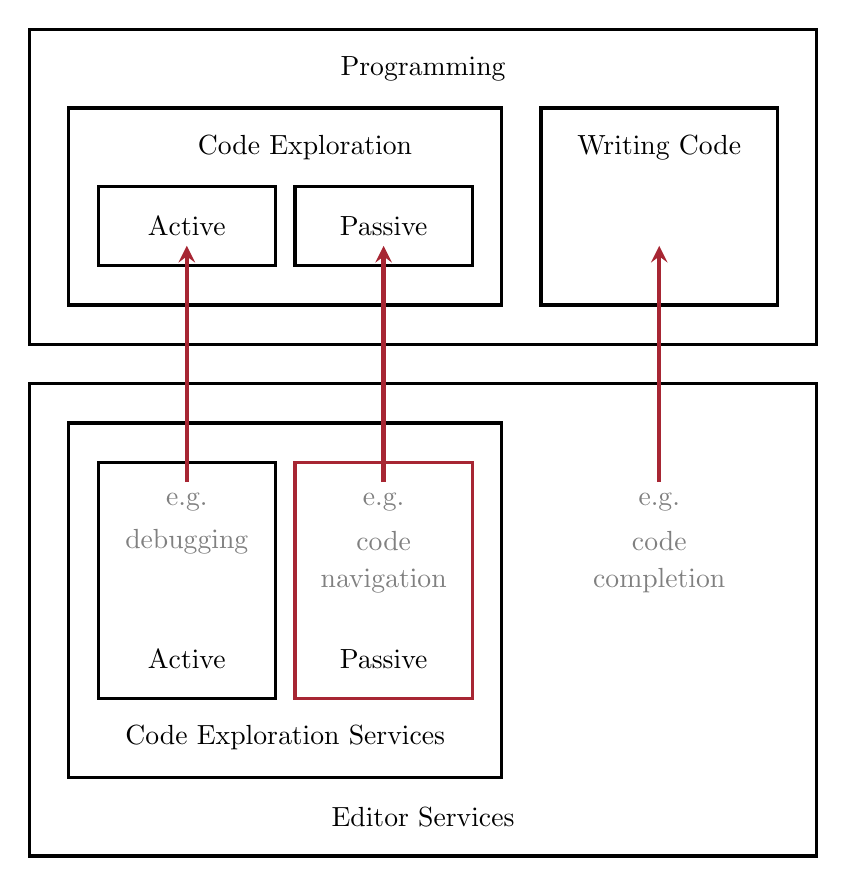
\begin{tikzpicture}[font={\xkcd}]

        \draw[very thick] (0, 6.5) rectangle (10,10.5);
        \draw (5,10) node {Programming};

        \draw[very thick] (0.5, 7) rectangle (6,9.5);
        \draw (3.5,9) node {Code Exploration};

        \draw[very thick] (0.875, 7.5) rectangle (3.125,8.5);
        \draw (2,8) node {Active};

        \draw[very thick] (3.375, 7.5) rectangle (5.625,8.5);
        \draw (4.5,8) node {Passive};


        \draw[very thick] (6.5, 7) rectangle (9.5,9.5);
        \draw (8,9) node {Writing Code};


        \draw[very thick] (0, 0) rectangle (10,6);
        \draw (5,0.5) node {Editor Services};

        \draw[very thick] (0.875, 2) rectangle (3.125,5);
        \draw (2,2.5) node {Active};

        \draw[very thick, draw={rgb:red,128;green,29;blue,39}] (3.375, 2) rectangle (5.625,5);
        \draw (4.5,2.5) node {Passive};

        \draw[very thick] (0.5, 1) rectangle (6,5.5);
        \draw (3.25,1.5) node {Code Exploration Services};

        \draw[-stealth, ultra thick, draw={rgb:red,128;green,29;blue,39}](2,4.75) -- (2,7.75);
        \draw[text=gray] (2,4.5) node {e.g.};
        \draw[text=gray] (2,4) node {debugging};

        \draw[-stealth, ultra thick, draw={rgb:red,128;green,29;blue,39}](4.5,4.75) -- (4.5,7.75);
        \draw[text=gray] (4.5,4.5) node {e.g.};
        \draw[text=gray] (4.5,4) node {code};
        \draw[text=gray] (4.5,3.5) node {navigation};

        \draw[-stealth, ultra thick, draw={rgb:red,128;green,29;blue,39}](8,4.75) -- (8,7.75);
        \draw[text=gray] (8,4.5) node {e.g.};
        \draw[text=gray] (8,4) node {code};
        \draw[text=gray] (8,3.5) node {completion};


    \end{tikzpicture}
    \caption{
        A visual overview of the definitions given in this section.
        Red arrows denote which kinds of services help with which kinds of programming tasks.
        Later on in the thesis, we will mostly be focussing on passive code exploration services, here depicted with a red outline.
    }
    \label{fig:definitions}
\end{figure}

%These services make navigation between various sources of information in and around the program quicker.
%There are also editor services that make active code exploration easier, like integrated debugging and testing.

%Diagnostic messages are an interesting in this regard.
%Do they help a programmer explore a program actively or passively?
%One way to gather diagnostic messages is by running for example a compiler of a language, and seeing what errors it gives.
%There are languages have turing complete type systems, allow arbitrary code to run at compile time, or lack a clear distinction between runtime and compile time.
%We might therefore say that diagnostic messages help with active code exploration.
%
%On the other hand, diagnostic messages are solely based on source code.
%While the diagnostic messages are generated, the programmer does not have to provide any inputs to the program.
%
%We, however, would not consider code exploration with the support of diagnostic messages active code exploration.
%The reason being that gathering diagnostic messages does not involve any interaction from the programmer.

%Although many editor services are useful for code exploration, some are not.
%For example, code completion is specifically aimed at writing code.
%Similarly, although formatted code might be easier to explore, the service of automatically formatting source code
%is not meant to make code exploration any quicker.

%The set of editor services which help with code exploration, we will from now on call code exploration services.
%Code exploration services form a subset of editor services, since any useful code exploration service can be useful in an editor,
%making that service also an editor service.

%Similar to the definition of code exploration, we can distinguish between passive and active code exploration services.
%Passive and active here refer to the kind of exploration the services help with, not necessarily the service itself.

\section{Code Exploration Services in other media}\label{sec:code-exploration-services-in-other-media}

Code exploration is always done in some environment, which we will call the code exploration medium.
Up to now, we have mainly discussed editors as a code exploration medium.
Because of the editor services many editors provide, editors are often a convenient code exploration medium.
However, editors are far from the \emph{only} code exploration medium.

For example, there are websites, such as \href{https://github.com}{github.com}, \href{https://stackoverflow.com}{stackoverflow.com} and a plethora of others which display code for users to explore.
Some websites even provide some of the services that editors also provide: the category we called code exploration services in the previous section.
Apart from websites, also PDF files (papers for example), presentation slides, books, videos, whiteboards and even verbal and written conversations might all be considered code exploration media as well,
which just like websites can support certain code exploration services.
For example, almost any medium, even those printed on paper, can have an outline or index, and syntax coloring.

Providing code exploration services in other media than editors is nothing new.
Many solutions already exist today, which do exactly that: simplifying code exploration by providing code exploration services.
To learn about what is possible in this space, we have made an overview of many important ones below.
We chose these tools, not simply based on popularity, but also to highlight interesting or relevant examples of code exploration services in
the field, to give a good overview of what options exist.

%However, all these examples of alternative code exploration media have certain limitations compared to an editor.
%This is not very surprising because an editor is essentially a purpose-built tool for code exploration.
%One limitation shared by almost all these media is that they cannot easily have users to run programs they are exploring.
%A website \emph{maybe} could allow that, and we will see an example that in \cref{sec:a-survey-of-existing-code-exploration-services}, but a book certainly cannot.

%That does not mean that these alternative code exploration media cannot provide certain code exploration services, making exploring code in them easier.

%As the name, implies, editor services are meant to be used in an editor.
%In an editor, editor services can help with code exploration.
%This raises the question, can editor services work in other code exploration media to make code exploration richer in those places as well?
%In that case, we might call the subset of editor services that are useful in other code exploration media as well, `code exploration services'.

% you can write code to explore other code. active vs passive code exploration
% maakt passieve code exploration services "richer"!

%\subsection{Limitations of code exploration media}\label{subsec:limitations-of-code-exploration-media}
%
%Providing editor services is often a dynamic process.
%As a programmer navigates and interacts with code, requests are made to some kind of server, which gives a response to the request.
%We discussed this in depth in section~\ref{subsec:language-servers}.
%For many media, such a dynamic system is simply out of the question.
%
%This is most apparent when targeting books or PDFs as exploration media, where providing anything dynamically is infeasible.
%Even on websites, where code can be run in real time, doing so for every user that explores the code can be costly and slow.
%Instead, one might want to analyze a source file (or group of source files) and output latex, or a static webpage with all the information in it.
%Even on a webpage, where information could feasibly be calculated dynamically, a statically generated page might still be beneficial.
%Multiple users who might see a webpage can then reuse the same analysis of the sourcecode.
%
%%\subsection{Making editor services more static}\label{subsec:work-towards-making-editor-services-more-static}
%%
%%In section~\ref{sec:an-overview-of-editor-services}, we saw places, which provide certain code exploration services.
%%To do this we saw that they gather information about sourcecode to statically provide information about that code later.
%%There have been attempts at making editor services more static than the very dynamic \ac{LSP}.
%%In this section we look at some of these attempts, and analyze how they work.
%
%\paragraph{Language Server Index}
%
%\paragraph{Jetbrains index format (PSI)}


%Code exploration services exist, in various forms, for different kinds of code exploration media, although different parties might give them different names.
%For example, in editors they are often grouped together with editor services, and GitHub does not give the group of
%services a name, but has a few independent services such as ``Code Navigation''\todo{ref}.
%In this section, we made an overview of places, which provide code exploration services, and evaluate what those places do.
%
%We chose these places, not simply based on popularity, but also to highlight interesting or relevant examples of code exploration services in
%the field, to give a good overview of what options exist.

\subsection{Documentation Generators}

To start off, many languages come with tools that can generate documentation.
Although their name suggests that they provide only a single editor service: ``documentation'', this is often far from true.
Instead, such tools often provide several code exploration services together, like code navigation, and syntax highlighting, though sometimes in limited form.
We will first look at some tools meant to serve only a single programming language or ecosystem, and then broaden our scope
to tools which are more widely applicable.

\paragraph{Rustdoc and other Single Language tools}

The standard Rust distribution ships with a tool called rustdoc~\autocite{rustdoc}.
The tool generate pretty documentation websites from Rust projects.
In a sense, it can be seen as a kind of compiler.
It takes Rust code, annotated with special comments (so-called doc-comments), and produces an HTML file.
The generated HTML contains only the documentation and public API of the code, not the code itself.

We can say that Rustdoc provides at least three code exploration services.
The main ones are documentation, and an outline.
Additionally, all parts of the public API are clickable, meaning there is also code navigation.
Finally, there are bits of code that are visible, mostly type signatures, which have coloured syntax.

Rustdoc is similar in many ways to tools such as Haddock for Haskell, Javadoc for Java, and countless comparable tools for other languages.

\paragraph{Agda to HTML and Latex}

Just like Rustdoc can generate documentation websites for Rust, the Agda compiler can produce HTML output based on Agda source code.
As we have seen, many languages have this capability, so although it can be useful, it is not especially novel.
However, we mention Agda separately because the language also natively supports generating LaTeX for use in papers~\autocite{agda_latex}.
The tool mainly performs syntax colouring.

\todo{Ask Jesper Why (because agda is often used for research and thus often part of papers?)}

\paragraph{Doxygen and CTAGS}

Doxygen~\autocite{doxygen} generates documentation pages just like Rustdoc does, and therefore seems quite similar in scope at first glance.
However, while Rustdoc only works for a single language: Rust and similarly Haddoc only works for Haskell, Doxygen actually supports quite a wide range of languages.
For example, C, C++ and Java, and with extensions even some less common languages are supported, as long as their syntax is somewhat similar to that of C.

Furthermore, Doxygen can produce all kinds of output formats, not just webpages.
Just like Agda, Doxygen supports outputting LaTeX, but also man pages and \acs{XML}.
The \ac{XML} output is interesting, because it is not intended to be human-readable, and instead captures the structure of programs in a more machine-readable format.

To provide code navigation in the generated documentation, Doxygen needs to have a way to figure out which parts of a codebase reference one another.
This is different for every language, and thus quite a complex task for a tool that aims to support many different languages.
All previously mentioned documentation generator tools have it much easier in this regard, they have only a single language to deal with.

To avoid this complexity, Doxygen uses a different program called CTAGS to generate reference information~\autocite{ctags}.
CTAGS is a tool that reads programs and codebases and generates so-called tagfiles.
Tagfiles are like a table of contents of a codebase, containing information about the location and type of all items in the codebase.

Such an index of definitions in a codebase is useful for all kinds of tools, not just Doxygen.
In fact, the main usecase of tagfiles is not Doxygen, but editors to help provide editor services.
Vim, for example, can read tagfiles to provide code navigation.

Although CTAGS can find identifiers in a source file, it does not understand scoping rules.
The result is that tools like Doxygen, that use CTAGS to provide code navigation, sometimes make mistakes.
If there are two items with the exact same name, Doxygen may refer to the wrong one or both.

Luckily, the languages that Doxygen works on have scoping rules that make triggering these mistakes somewhat difficult.
For example in C++, toplevel items are not allowed to shadow each other.
Still, it is possible to carefully craft an example that shows Doxygen making mistakes in finding what parts of the program reference what other parts.
We used Doxygen to generate documentation for the C++ code snippet below, in which both the enum variant \texttt{A::X} and the struct \texttt{X} are in global scope:

\begin{lstlisting}
#include<iostream>

enum A {
    X = 5,
};

struct X {};
const A x = X;

int main() {
    std::cout << x << std::endl;
}
\end{lstlisting}

In C++, you do not need to qualify usage of an enum variant, so on line 8, the variable \texttt{example} gets the value $5$ assigned which is printed in \texttt{main}.
However, Doxygen internally thinks that the enum variant is called \texttt{A::X} and the struct is just called \texttt{X}.
Therefore, the \texttt{X} in \texttt{const A x = X} does not \emph{exactly} match the enum variant name and instead Doxygen thinks this statement refers to the struct \texttt{X}, the name of which \emph{does} match exactly.
Doxygen shows this association by generating a blue link, and in \cref{fig:mistake-in-doxygen} the arrow shows where the link (mistakenly) takes users.

\begin{figure}[!h]
    \centering
    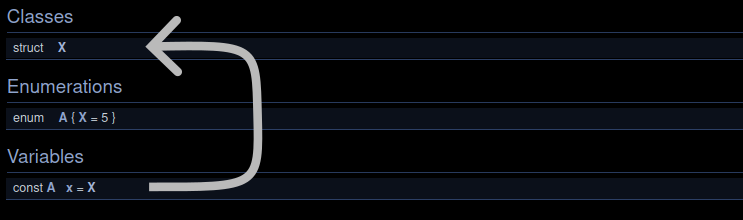
\includegraphics[width=\textwidth]{../images/doxygen-output}
    \caption{
        Doxygen links from \texttt{const A x} to \texttt{struct X} because it wrongly matches the value to the struct which is also named \texttt{X}.
        Doxygen should instead link to the variant named \texttt{X} in \texttt{enum A}.
        The white arrow shows where the blue \emph{X} link points users to.
    }
    \label{fig:mistake-in-doxygen}
\end{figure}

\paragraph{CBS}

For a language called CBS, short for Component Based Semantics, a system was created to generate a documentation website based on source code~\autocite{Mosses19}.
The tool is currently a single-language tool like others we discussed in this section, and also like other tools it can generate LaTeX source code as well.
What is different, is that CBS is built with the Spoofax language workbench.
In \cref{subsec:language-workbenches}, we discussed the possibilities language workbenches possess to provide editor services across a wide range of languages.
and this is also the goal for CBS' documentation generator as \citeauthor{Mosses23} states in \citetitle{Mosses23}\autocite*{Mosses23}.

\subsection{Collaboration}

In this section, we will discuss a few notable tools out of many that aid programmers collaborating while writing programs.
The ones we will discuss are web-based, and on many pages of their website code is displayed.
It is not always convenient to download this code to a local development environment to run and explore it in an editor.
Therefore these websites provide various online code exploration services of differing sophistication.

\paragraph{StackOverflow}

The first somewhat noteworthy tool is StackOverflow.
The code exploration services StackOverflow provides are rather limited.
Although many programmers look for code on the website, they essentially only provide programmers with syntax colouring, and that might just be plenty for the purposes of the site.

StackOverflow is based on questions and hand-written answers by other programmers.
Answers may contain snippets of code to explain a certain concept without requiring much further context.
Providing more than syntax colouring for these small snippets is likely difficult and may not even be very helpful for users.

What may happen though, is that the question that somebody asked on StackOverflow does not exactly match the one you have.
As such, the given answer might not work for you.
In that case, you could ask your own question, but StackOverflow also has a built-in service that finds related questions that might match your question better.
One could argue that this is a form of code navigation, although not based on the contents of programs and instead based on the meaning of the code.

\paragraph{GitLab and GitHub}

In contrast to StackOverflow, GitLab is often used to store entire projects, not just snippets of code.
GitLab is a platform with which people can collaborate on projects using Git, a version control system.
To help people explore code on their platform, GitLab performs Code Colouring for many languages when viewing files with source code in them.
Additionally, GitLab has search functionality that can be scoped to a particular project or group of projects.

Search features were not part of the editor and code exploration services described in \cref{sec:an-overview-of-editor-services}, and we will discuss this further in \cref{sec:code-search}.

\begin{figure}[!h]
    \centering
    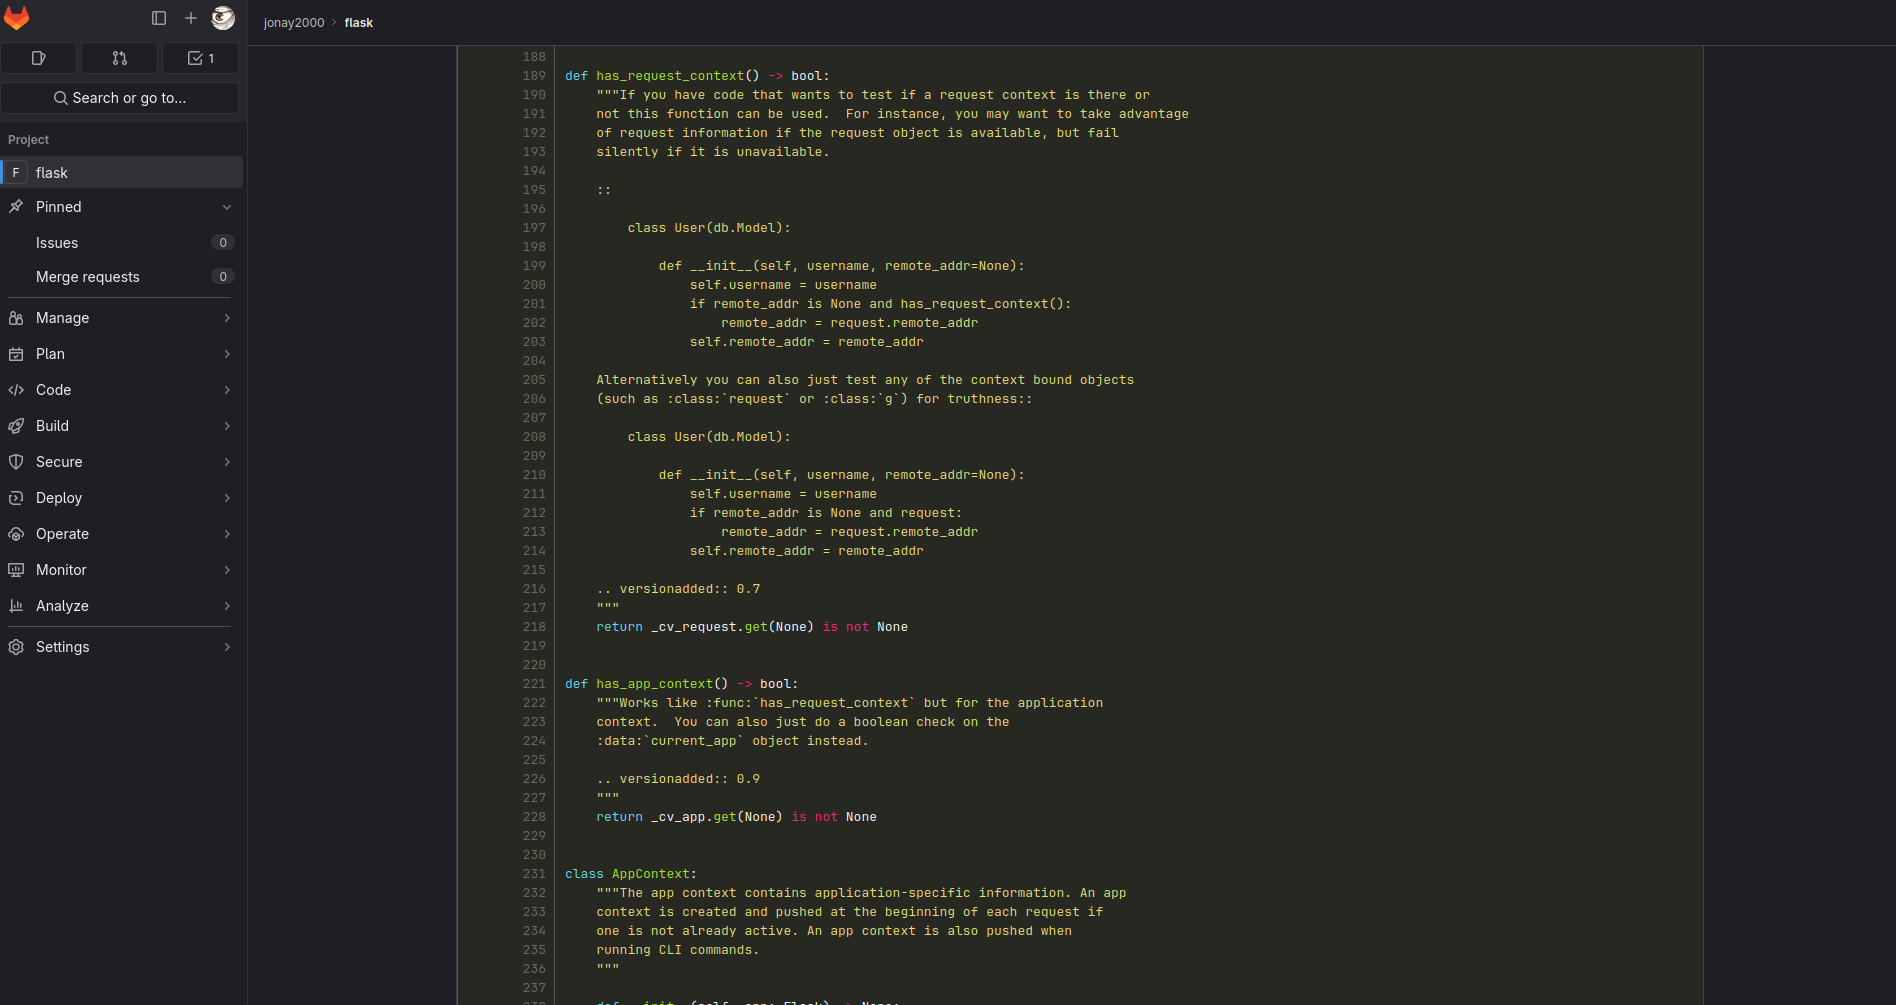
\includegraphics[width=\textwidth]{../images/flask-gitlab}
    \caption{\textit{context.py} from the Python Flask repository viewed on GitLab with only syntax Colouring.}
    \label{fig:flask-on-gitlab}
\end{figure}


GitLab provides few code exploration services compared to GitHub, a platform that provides similar features to GitLab.
Just like on GitLab, programmers often upload entire codebases to GitHub, and work on their code together through Git.
However, GitHub gives us a taste some of what is possible with more advanced Code Exploration Services.

In addition to the quite standard Code Colouring, GitHub, allows visitors of the site to easily navigate source code of
certain programming languages (such as Python) by jumping from usages to definitions and back, even between different files of a project.
Instead of depending on exact name matches like Doxygen does, GitHub builds a model of the scoping rules of a language using Stack Graphs~\autocite{CreagerA23, stackgraphs}.
Based on this model, they can work out which identifiers refer to which other identifiers while taking scoping rules into consideration.

In~\cref{subsec:language-workbenches}, we discussed language workbenches and Spoofax.
To define the scoping rules of a language in Spoofax, a model called Scope Graphs is used~\autocite{NeronTVW15, AntwerpenNTVW16, AntwerpenPRV18}.
Stack Graphs are based on, Scope Graphs, but modified to be highly incremental.
That means that when someone changes one file in the project, by making a Git commit, GitHub does not have to re-analyse all other files in the code base.

In \cref{fig:flask-on-github} we provided a demonstration of code navigation through the Python Flask project based on Stack Graphs on Github.
At the time of writing, GitHub has only enabled Stack Graphs based navigation for Python, though the plan is to provide this for more languages~\autocite{CreagerA23}.

\begin{figure}[!h]
    \centering
    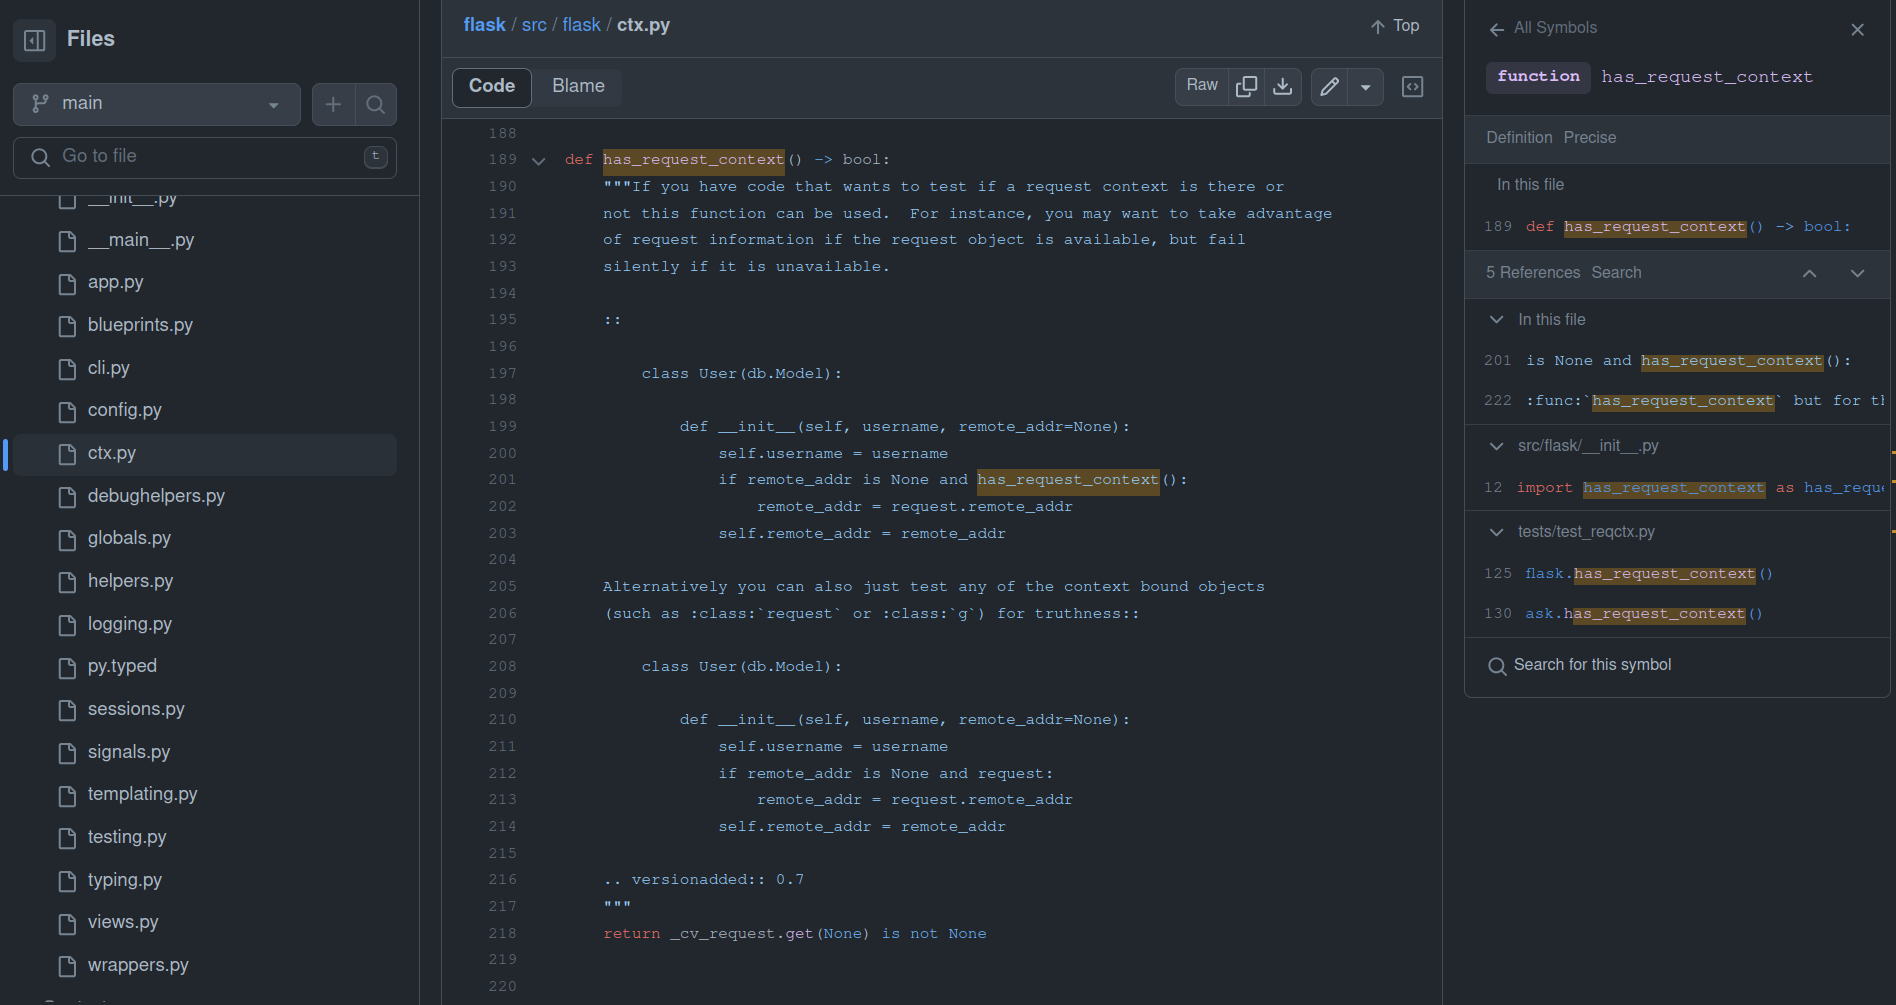
\includegraphics[width=\textwidth]{../images/flask-github}
    \caption{
        The same \textit{context.py} as shown in~\cref{fig:flask-on-gitlab} from the Python flask repository on GitHub,
        showing a file overview on the left, coloured code in the middle with one identifier selected: \texttt{has\_request\_context}.
        On the right, the code navigation menu is open (which happens after an identifier is selected) showing navigation options:
        two in this file and 3 more in different files. Clicking these options navigate to those files in the browser.
    }
    \label{fig:flask-on-github}
\end{figure}

In addition to Syntax Colouring, Code Navigation (for Python) and extensive search options, GitHub users
have also found custom ways to add limited diagnostics messages to code displayed on the site.
For example, the \url{https://github.com/actions-rs/clippy-check} automatically checks code uploaded to project repositories on GitHub
by using GitHub Actions, GitHub's continuous integration service, and adds comments at the places where warnings and errors are found.


\subsection{Other tools}

Finally, there are several tools which do not fit any specific category, and yet are certainly worth a mention.

\paragraph{Web Code Colourers}
First, there are several JavaScript libraries which specifically solve syntax colouring on websites.
For example, there are \textcite{highlightjs} and \textcite{prismjs}, which essentially package a single code exploration service: code colouring, to work for hundreds of languages on any website.
Several of the websites we discussed sofar use highlight.js on their website, like StackOverflow and GitLab~\autocite{so_highlightjs, gl_highlightjs}, while, for example, GitHub uses a custom system.

\paragraph{LaTeX Code Colourers}

Next, there are similar tools that provide syntax colouring in LaTex documents.
Since this thesis was written using LaTeX, we can demonstrate those in this document.
First, there's the LaTeX \texttt{listings} package, which simply highlights a number of predefined keywords as the example below shows.

\begin{lstlisting}[language=rust]
fn fibonacci(n: u64) -> u64 {
    match n {
        0 => 0,
        1 => 1,
        n => fibonacci(n - 1) + fibonacci(n - 2)
    }
}
\end{lstlisting}

Which keywords are highlighted changes per language, and users of the library can define their own set of keywords that should be highlighted.
This is different to what the LaTeX \texttt{minted} package does, which uses an external tool called \citetitle{pygments}~\autocite*{pygments} to perform highlighting.
The result looks a lot more like what web-based code listings look like.

\begin{minted}{rust}
fn fibonacci(n: u64) -> u64 {
    match n {
        0 => 0,
        1 => 1,
        n => fibonacci(n - 1) + fibonacci(n - 2)
    }
}
\end{minted}

\paragraph{Bootlin}

\todo[inline]{Short explanation here}

\paragraph{Matt Godbolt's Compiler Explorer}
The Compiler Explorer is an online tool created by Matt Godbolt, available at \url{https://godbolt.org}.
On the website, users can write code in a simple editor and execute it (non-interactively) on the server, and this works for a large range of different compiled programming languages.
This makes the compiler explorer, in contrast to the other systems in this list in that it also provides active code exploration services: users can see what their code does when ran.

Furthermore, the compiler explorer is more than just an online editor and few people would use it as such.
The main purpose of the Compiler Explorer is instead to be able to choose \emph{exactly} what compiler is used to compile the code.
The website can, instead of running the code, also give the binary and assembly output of the compiler, and link each line in the source code to what assembly instructions correspond to it.
With the compiler explorer, users can research differences in the code generated between different compilers and programming languages

\subsection{Evaluation}\label{subsec:evaluation}

In this section we have discussed many examples of systems that provide a wide range of code exploration services in several media.
However, many of the discussed approaches are quite narrow in scope.
For example, they support:
\begin{enumerate}
    \item only one single, or small number of languages, like the documentation generators we discussed and even GitHub's Stack Graphs which at this moment only supports Python.
    \item only a single code exploration medium.
    For example, the Rust library called stack-graphs that powers GitHub's code navigation is open source, GitHub's integration on their website is closed source and cannot easily be replicated on other websites.
    That means that GitHub's solution is mostly restricted to GitHub.
    \item only a single code exploration service is supported.
    For example, the code colouring systems we have looked at, or the documentation generators (which are thus narrow in two different ways), and also GitHub's Stack Graphs which is only made to provide code navigation.
\end{enumerate}

What we see here is, in essence, similar to the IDE portability problem described in \cref{sec:ide-portability-problem}.
There are $m$ languages for which services are provided in $n$ places and no party can feasibly be responsible for those \problem{\times} implementations.
Instead, many narrow solutions form the landscape of code exploration services in various media.
We call this, the \problem{\times} problem for code exploration services, and in the rest of this thesis we will be working towards a solution for this problem.
A solution which is not as narrow and can, in a language-agnostic manner support multiple kinds code exploration services, in multiple code exploration media.


\todo[inline]{not narrow = has butterfly shape}

%\section{Towards generic code exploration services}
%
%As we showed in section~\ref{sec:a-survey-of-existing-code-exploration-services}, many parties try to provide editor services
%at a limited capacity.
%This creates a \problem{\times} problem, where $m$ parties try to implement services for $n$ languages.
%Then, in section~\ref{sec:}, we mentioned different kinds of code exploration media that might
%want to give outputs based on an analysis of sourcecode.
%Again, this would be $M$ media, which might want to support $N$ languages.
%
%To solve this problem, we hypothesise that we need a unifying interface, just like the \ac{LSP} or \ac{AESI}, between code exploration media
%and sourcecode.
%This interface cannot be like a protocol.
%As we established, unlike with the \ac{LSP}, it is often not feasible, nor necessary to have a server that can
%dynamically communicate with the client.
%
%Instead, we think that the solution is a kind of index format, in a sense a static version of the \ac{LSP}.
%A format that can be generated out of various sources, and that can be interpreted to generate various code exploration media
%with code exploration services embedded.
%A kind of intermediate format that can contain static analyses for any programming language.
%
%To actually create such a format, and to find out whether or not such a data format is really the best solution to the problem we discussed,
%we aim to find answers to the following questions:
%
%% what is a good index format for ...
%% Specific about contributions, base questions on these
%
%\begin{itemize}
%    \item Can we create an index format for language-parametric code exploration services.
%    \item How can an index format for language-parametric code exploration services be created.
%    \item (What considerations should be taken when creating an index format for language-parametric code exploration services.)
%    \item What are alternatives to an index format for language-parametric code exploration services, and how do the alternatives compare to an index format.
%\end{itemize}
%
%%\todo[inline]{Somewhere write about what such a format can actually be used for. I don't know what the best spot for that is, either
%%after I introduced that we think a format is useful, or before as a motivation for such a format. Many applications will be
%%the existing CES mentioned in the survey, but we can also be more broad and relate it to educative purposes for example.
%%
%%--> Introduction
%%}
